\documentclass{article}

\usepackage{fontspec}   %加這個就可以設定字體
\usepackage{xeCJK}       %讓中英文字體分開設置
\usepackage{indentfirst}
\usepackage{listings}
\usepackage{minted}
\usepackage{float}
\usepackage{graphicx}
\usepackage{fancyhdr}


\usepackage[
  top=2cm,
  bottom=2cm,
  left=2cm,
  right=2cm,
  headheight=17pt, % as per the warning by fancyhdr
  includehead,includefoot,
  heightrounded, % to avoid spurious underfull messages
]{geometry} 



\pagestyle{fancy}

\lhead{P vs NP}
\rhead{武陵資訊讀書會}

\cfoot{\thepage}
%\rfoot{李杰穎}

\lstset{basicstyle=\ttfamily, keywordstyle=\bfseries}

\setCJKmainfont{Noto Sans CJK TC}
\XeTeXlinebreaklocale "zh"             %這兩行一定要加,中文才能自動換行
\XeTeXlinebreakskip = 0pt plus 1pt     %這兩行一定要加,中文才能自動換行
\title{P vs NP}
\author{Jayinnn aka 李杰穎}
\date{\today} %不要日期

\setlength{\parindent}{2em}
\setlength{\parskip}{1em}


\renewcommand{\thefootnote}{\roman{footnote}}

\begin{document}
\maketitle
\section{前言}

今天是第一次的資訊讀書會,應該蠻有紀念意義的ㄅ

資訊讀書會,我目前規劃是說程式語言的部份教的少一點,專注在演算法方面,因為我覺得程式語言其實不太好教,但如果大家想要的話我是可以教拉,今天上課後可以跟我講一下我收集一下意見。

\section{時間複雜度(Time complexity)}
就是一個函數,描述一個演算法的執行時間。

簡單來說,假設有一個演算法,你給這個演算法一個大小為n的輸入,它最多要 $6n^3+5n^2+2n+1$ 的時間才能執行完畢,我們就說這個演算法的時間複雜度是$O(n^3)$,這個$O()$我們稱作大O符號 (Big O notation),又叫做漸進符號,它是用另一個(通常更簡單的)函式來描述一個函式數量級的漸近上界。

還有一個東西叫做最壞時間複雜度(Worst-case complexity)記作 $T(n)$

排序演算法的其中一種:插入排序(insertion sort)的時間複雜度是$O(n^2)$,下面是插入排序的Python 程式,為什麼這個演算法的是$O(n^2)$嗎?

\begin{minted}{python}
def insertionSort(arr):   
    # Traverse through 1 to len(arr)
    for i in range(1, len(arr)):   
        key = arr[i]   
        # Move elements of arr[0...i-1],        
        while j >= 0 and key < arr[j] : 
                arr[j+1] = arr[j] 
                j -= 1
        arr[j+1] = key 
\end{minted}

我們今天不會提到太多的排序演算法,因為我們的主題是P vs NP。

\section{P}
P 代表的是 Polynomial (多項式),若有一個問題可以在多項式時間(polynomial time)複雜度\footnote{$O(1), O(\log n), O(n^2), O(n \log n), O(n^3), O(n^4)$...皆為多項式時間複雜度}解決,則我們說此問題為P類問題。

\subsection{最大值問題}
給定一個序列,裡面包含一堆整數,求此序列最大值?

這個問題顯然是$O(n)$,所以我們可以說 $\mbox{maximum problem} \in P$

Python:
\begin{minted}{python}
def maximum(a):
    Max = a[0]
    for item in a:
        if item > Max:
            Max = item
            
    return Max
\end{minted}

C++:
\begin{minted}{C++}
int maximum(int arr[], int len){
    max = arr[0];
    for(int i = 1;i < len;i++){
        if(arr[i] > max){
            max = arr[i];
        }
    }    
    return max
}

\end{minted}


\section{NP}

NP 並不是 non-polynomial 的縮寫,而是 non-deterministic (非決定性) polynomial (多項式)。

如果一個問題可以在多項式時間內確定一個解是不是這個問題的解,則我們就說這個問題是NP類問題。

很顯然的,所有$\in$P的問題,一定也$\in$NP,所以P$\subset$NP。

\subsection{最大值問題}
最大值問題顯然$\in$ NP,確定其解的時間複雜度為 $O(n)$

\subsection{中位數問題}
給你一個序列,求其中位數。

這個問題$\in$ P\footnote{時間複雜度為$O(n \log n)$},且也 $\in$ NP\footnote{時間複雜度為$O(n)$}

\section{NP Hard}
NP Hard的非正式定義是:至少和NP中最難的問題一樣難。更正式一點的定義是,如果所有NP問題都可以在多項式時間歸約(Reduction)到某一個問題H,則我們就說問題H是NP Hard (NP 困難)的。

如果一個問題X可以在多項式時間內歸約成問題Y,我們可以記作$X\leq _{P}Y$。所以只要解出問題Y,我們就可以利用這個解去解問題X。

注意一下,NP Hard不一定是NP問題喔。

像等等會提到的子集和加總和3-SAT問題就是NP Hard問題。

\section{NP Complete}
若一個問題$\in$NP,且也$\in$NP Hard,這我們稱這個問題為NP完全問題 (NP Complete)。這類問題是最不可能被化簡為P的集合。很多人一開始會把NP的概念與NP Complete概念搞在一起,所以要注意一下。

下面幾個例子就是NP Complete的
\subsection{子集合加總問題}
給定一個有限數量的整數集合,找出任何一個此集合的非空子集且此子集內合為零。

暴力法複雜度為$O(2^n)$

DP算法\footnote{動態規劃(Dynamic Programming)以後有機會應該會提到}複雜度為$O(n(P-N))$\footnote{P是這個整數集合所有正數的和,N為所有負數的和}

\begin{minted}{C++}

// Returns true if there is a subset of set[] with sun equal to given sum
bool isSubsetSum(int set[], int n, int sum) {
    // The value of subset[i][j] will be true if there is a subset of set[0..j-1]
    //  with sum equal to i
    bool subset[sum+1][n+1];
 
    // If sum is 0, then answer is true
    for (int i = 0; i <= n; i++)
      subset[0][i] = true;
 
    // If sum is not 0 and set is empty, then answer is false
    for (int i = 1; i <= sum; i++)
      subset[i][0] = false;
 
     // Fill the subset table in botton up manner
     for (int i = 1; i <= sum; i++)
     {
       for (int j = 1; j <= n; j++)
       {
        //
         subset[i][j] = subset[i][j-1];
         if (i >= set[j-1])
           subset[i][j] = subset[i][j] || subset[i - set[j-1]][j-1];
       }
     }
 
 
     return subset[sum][n];
}
\end{minted}

\subsection{3-SAT}
假設有一堆boolean\footnote{布林值,可以簡單想成只有1(True)和0(False)的資料型態} $x_1, x_2, x_3, \ldots, x_n$,然後將這些boolean 組成 CNF (Conjunctive Normal Form) 的形式。
\begin{equation}
\Phi = (x_1 || !x_2 || x_3) \&\& (!x_2 || !x_4 || x_5) \&\& (x_1 || !x_3 || x_5) \&\& (x_2 || x_6 || !x_7)
\end{equation}
3-SAT 問題就是問說有沒有一種布林值的組合,使得這些由一大堆boolean所組成的CNF的最終結果為True。很顯然我們可以在$O(1)$就可以驗證一組數值是否為3-SAT問題的解,所以它$\in$NP。但我們目前沒有一個演算法可以在多項式時間搞定這個問題,目前唯一的算法只有將所有組合列出來,一個一個帶入原式,這樣的時間複雜度為$O(2^n)$,為指數時間,所以3-SAT問題$\not\in P$,而且我們等等會提到幾個NP問題的例子,我們會發現這些問題都可以在多項式時間歸約到3-SAT問題。

綜合以上3-SAT是一個NP Complete問題。

\begin{figure}[h]
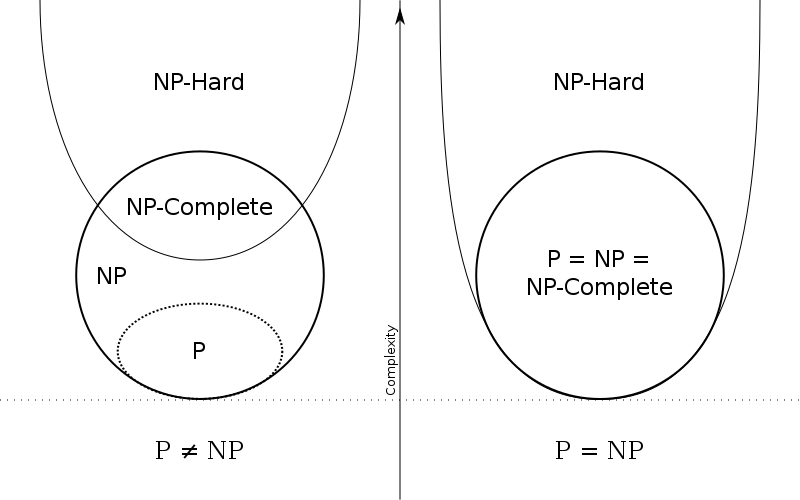
\includegraphics[width=\textwidth]{PNP.png}
\caption{描述P, NP, NP完全,以及NP困難之間關係的歐拉圖}
\end{figure}

\section{P = NP?}

P/NP問題是在理論資訊學中計算複雜度理論領域裡至今未被解決的問題,也是克雷數學研究所七個千禧年大獎難題之一。

但這個問題從1971年被史提芬·古克(Stephen A. Cook)和Leonid Levin提出後,到目前仍沒有解答。

剛剛提到的問題有些$\in$NP,但目前暫時$\not\in$P,P=NP問題想要問的就是:是不是所有$\in$NP的問題,都$\in$P,換句話說,P這個集合是否等於NP。

我們剛剛提到NP Complete在這個問題的證明非常有用,因為只要任何一個NP Complete問題被證明出來$\in$P,基本上就能確定P=NP。

很不幸的,現在有一堆問題是NP Complete,但沒有一個問題被證明出來$\in$P。

接下來會介紹一堆NP問題,還有它怎麼在多項式時間轉換成3-SAT問題。


\section{CLIQUE問題}
給你一個圖,給定一個數字k,問是否可以在這張圖找到一個子圖,其節點數恰好為k,且為全連接圖。

3-SAT問題可以被歸約成CLIQUE問題,也就是說 3-SAT$\leq _{rm P}$CLIQUE

\section{Independent Set問題}
給定一個圖,與一個數字k,問是否可以找到k個不相鄰且相異的點

同樣的,3-SAT問題可以被歸約成Independent Set問題,也就是說 3-SAT$\leq _{\rm P}$ Independent Set

\section{Vertex Cover問題}
給定一個圖,與一個數字k,問是否可以找到k個相異點,使這k個點可以覆蓋到此圖中所有的邊。

同樣的,3-SAT問題可以被歸約成Vertex Cover問題,也就是說 3-SAT$\leq _{\rm P}$ Vertex Cover

\end{document}

